\section{Data Structure for Representing Hierarchy of Clusters}
\label{sec:data_structure}

In this section we describe a data structure that can record the solution of an agglomerative
clustering algorithm efficiently, namely, with linear space complexity, by providing the following function:
\begin{itemize}
	\item \merge{$i$,$j$,$`g$} runs in $O(\log n)$ time and
	merges nodes $i,j\in V$ into the same cluster for all threshold values $<`g$.
\end{itemize} 
An agglomerative clustering algorithm should call \merge successively with distinct pairs of nodes and 
non-increasing values of $`g$. After all the nodes are merged into the trivial cluster $V$, the
following functions can be used to retrieve information about the clusters in linear/sub-linear
time:
\begin{itemize}
	\item \getCriticalValues{} runs in $O(n)$ time and returns the ordered list of critical threshold
		values $`g_{\ell}$'s in \eqref{eq:PSP} where the set of clusters changes.
	\item \getPartition{$`g$} runs in $O(n)$ time and returns the partition $\mcP$ of $V$ such that
		$\pzC_{`g}(\RZ_V)=\mcP`/\Set {\Set {i}\mid i\in V}$. In other words, $\mcP$ is the partition
		$\mcP_{\ell}$ in \eqref{eq:PSP} with the smallest $`g_{\ell}\geq `g$.
	\item \similarity{$i$,$j$} runs in $O(\log n)$ time and returns the critical value at which nodes $i,j\in V$ no longer belong to the same cluster, i.e., the largest critical value $`g_{\ell}$ s.t. $i$ and $j$ belong to the same cluster for all thresholds $\gamma' < `g_{\ell}$.

\end{itemize}

Internally, the hierarchy of clusters is represented by a weighted rooted tree on $V$, in which each
node $i\in V$ is associated with the following data:
\begin{itemize}
	\item \Parent{i}: The parent of $i$. If $i$ has no parent, then \Parent{$i$}$=i$.
	\item \Children{i}: The list of children of $i$. If $i$ has no children, then the list is empty.
	\item \Weight{i}: The weight of the edge between $i$ and its parent. It is initialized to $-`8$.
	\item \Rank{i}: The depth of the maximal subtree rooted at $i$. It is initialized to $0$.
\end{itemize}
\figref{fig:data_structure} gives the pseudocode of all the functions that support the desired data structure. The idea is to represent clusters by a weighted tree $T$ where each
edge $\Set {i,j}\in \mcE(T)$ has certain real-valued weight. %a weight $w(\Set {i,j})\in `R$:

\begin{Definition}
\label{def:data-structure}
	Given a tree $T$, the set of clusters at threshold $`g$ is the set $\mcP(T_{`g})`/\Set {\Set {i} \mid i\in V}$ of
	connected components of the forest $T_{`g}$ obtained from $T$ by removing edges of weights $\leq
	`g$.
\end{Definition}

The function \initialize constructs the leaves, namely, the singleton subsets $\Set{i}$ for $i\in V$.
To construct $T$ starting from its leaves, we call the function \merge{$i,j,`g$} for some $i,j,`g$, which verifies if $i$ and $j$ are already connected in $T$, and
if not, adds an edge with weight $`g$ between any node $i'$ connected to $i$ and any node $j'$
connected to $j$.
(A more specific choice of $i'$ and $j'$ will be discussed shortly.)
The computational complexity is $O(\log n)$ if the verification of connectedness can be
done in $O(\log n)$ time. This can be done using the same idea as the disjoint-set forest 
with union by rank~\cite{galler64,tarjan84}, by providing the function: 
\begin{itemize}
	\item \find{$i$} that runs in $O(\log n)$ time and returns a representative of the component containing $i$.
\end{itemize}
%Assuming two nodes in the same connected components have the same representative, 
Then, node $i$ is connected to node $j$ iff \find{$i$}$=$\find{$j$}.
%, which can be checked in $O(\log n)$ time as desired.
To implement \find, with the desired $O(\log n)$ complexity, the partial clustering solution is represented by a rooted
forest where each connected component is a rooted tree and so \find can simply return the root of
the tree as the representative of the component.
%Let $i'$ and $j'$ be the roots of the components containing $i$ and $j$, respectively.
To maintain the invariance that the graph is a
rooted forest, \merge{$i,j,`g$} adds a edge with weight $`g$ between the root $i'$ of $i$
and the root $j'$ of $j$ if $i'\neq j'$. To ensure $O(\log n)$ complexity for \find and therefore
\merge, the root of the deeper tree is chosen to be the parent of the other root since this 
ensures that the depth of any tree in the forest to be $O(\log n)$ at all times. Note that, different from \cite{felzenszwalb2004efficient}, the path compression technique for disjoint-set forest cannot be adopted here as it would destroy the hierarchical structure. 

\begin{figure}
	{%\scriptsize
		\setlength{\algomargin}{0.4em}
		\noindent\begin{minipage}[t]{.45\linewidth}
			\begin{algorithm}[H]
				\myfn(\label{ln:initialize}){\initialize{}}{
                	\For{$i\in V$}{
                		\Parent{$i$}$"<-"i$,
                		\Children{$i$}$"<-"$empty list,
                		\Weight{$i$}$"<-"-`8$,
                		\Rank{$i$}$"<-"0$;\;
                    }
            	}
            	\BlankLine
				\myfn(\label{ln:find}){\find{$i$}}{
					\lIf{\Parent{$i$}=$i$}{
						\KwRet $i$;
					}
					\lElse {
						\KwRet \find{\Parent{$i$}};
					}

				}
				\BlankLine
				\myfn(\label{ln:merge}){\merge{$i$,$j$,$`g$}}{
					$i'"<-"$\find{$i$},
					$j'"<-"$\find{$j$};\;
					\lIf{$i'$=$j'$}{\KwRet;}
					\uIf{\Rank{$i'$} $\leq$ \Rank{$j'$}}{
						\Parent{$i'$}$"<-"j'$;\;
						add $i'$ to \Children{$j'$};\;
						\Weight{$i'$}$"<-"`g$;\;
						\lIf{\Rank{$i'$}$=$\Rank{$j'$}}{
						\Rank{$j'$}$"<-"$\Rank{$j'$}+1;
						}
					}					
					\Else {
						\Parent{$j'$}$"<-"i'$;\;
						add $j'$ to \Children{$i'$};\;
						\Weight{$j'$}$"<-"`g$;\;
					}
				}
			\end{algorithm}
		\end{minipage}
		\begin{minipage}[t]{.45\linewidth}
			\begin{algorithm}[H]
				\myfn(\label{ln:getCriticalValues}){\getCriticalValues{}}{
					%\KwIn{}
					%\KwOut{}
					%\BlankLine
					\KwRet \DataSty{weight};\;
				}
				\BlankLine
				\myfn(\label{ln:getPartition}){\getPartition{$`g$}}{
					$S"<-"V$, $\mcP"<-"`0$;\;
					\While{$S\neq `0$}{
						$i"<-"$ any node from $S$;\;
						$B"<-"$ set of nodes reachable from $i$, by going from a reachable node $j$ to \Parent{$j$} if \Weight{$j$}$>`g$ and to $j'\in$\Children{$j$} if \Weight{$j'$}$>`g$;\;
						$S"<-"S`/B$, add $B$ to $\mcP$;\;
					}
				}
				\BlankLine
				\vspace{.4em}
				\myfn(\label{ln:similarity}){\similarity{$i$,$j$}}{
					\lIf{$i=j$}{\KwRet $`8$;}
					$i'"<-"$\Parent{$i$},
					$j'"<-"$\Parent{$j$},
					$`g_i"<-"$\Weight{$i$},
					$`g_j"<-"$\Weight{$j$};\;
					\lIf{$i'=j$}{\KwRet $`g_i$;}
					\lIf{$j'=i$}{\KwRet $`g_j$;}
					\uIf{$`g_i \geq `g_j$}{ 
						\KwRet \similarity{$i'$,$j$};\;
					}
					\lElse{
						\KwRet \similarity{$i$,$j'$};
					}

				}
			\end{algorithm}
		\end{minipage}
	}
	\caption{Pseudocode to construct (left) and query (right) the data structure for the clustering solution.}
	\label{fig:data_structure}
\end{figure}

Finally, using the data structure described above, the agglomerative info-clustering algorithm in Algorithm~\ref{alg:aic} and \ref{algo:fuse} can be implemented as shown in Algorithm~\ref{algo:aic-tree}.

\begin{algorithm}
	\caption{Implementation of Agglomerative info-clustering using an efficient data structure.}
    \label{algo:aic-tree}
	\BlankLine
	%\KwData{$\mcP_{\ell}, \mcP_{\ell+1}, \dots, \mcP_{N}$ in \eqref{eq:PSP} for some $1\leq \ell \leq N$ have been recorded by the data structure.}
	%\KwResult{$\mcP_{\ell-1}$, if any, i.e., $\ell>1$, is recorded by the data structure.}
	\KwData{Statistics of $\RZ_V$ sufficient for calculating the entropy function $h(B)$ for
	$B\subseteq V:=\{1,\ldots,n\}$.}
	\KwResult{Info-clustering solution in Proposition~\ref{prop:clusters} recorded by \Parent, \Children, \Weight and \Rank.}
	\initialize{};\;
	$\mcP\leftarrow$\getPartition{$-\infty$};$k\leftarrow \abs{\mcP}$;\;
	\While{$k>1$}{
    	\DataSty{x}$\leftarrow$ empty array of size $k$;\;
    	\For{$j\leftarrow 1$ \emph{\KwTo} $k$ }{
    		%\DataSty{x}[$j$]=\MinNormBase($ B\mapsto h`1(\bigcup_{i\in B\cup\Set{j}}C_i`2)-\sum_{i\in B\cup\Set{j}}h(C_i),\Set{j+1,\ldots,k}$);\; \label{ln:MNB:1}
    		Define $g_j$ as the function $ B\subseteq \{j+1,\dots,k\}  \mapsto h`1(\bigcup_{i\in B\cup\Set{j}}C_i`2)-\sum_{i\in B\cup\Set{j}}h(C_i)$;\; 
    		\DataSty{x}[$j$]$\leftarrow$\MinNormBase($g_j,\Set{j+1,\ldots,k}$);\; %\label{ln:MNB:1}
    	}
    	%\KwRet $(\upgamma_1(\RZ_B),\pzC_{\upgamma_1}(\RZ_B))$;
    	$\displaystyle`g\leftarrow -\min_{i,j:1\leq j<i\leq k}\DataSty{x}[j][i]$;\;
    	\For{$j \leftarrow 1$ \emph{\KwTo} $k$ }{
    	    \For{$i \leftarrow 1$ \emph{\KwTo} $j-1$ }{
        		\If{$\DataSty{x}[j][i]\kern-.25em\leq\kern-.25em -`g$}{
        			\merge{$u$,$v$,$`g$} for an arbitrary $u\in C_i$ and an arbitrary $v\in C_j$;\; 
        			%add $C_j \cup \bigcup\Set{C_i\mid i\kern-.25em\in\kern-.25em\Set{j\kern-.25em
        			%+\kern-.25em 1,\dots,k}, \DataSty{x}[j][i]\kern-.25em\leq\kern-.25em -`g}$ to $\mcP'$;\;
        		}
    		}
		}
		$\mcP\leftarrow$\getPartition{$-\infty$};$k\leftarrow \abs{\mcP}$;\;
	}
\end{algorithm}
    
The following example demonstrates Algorithm~\ref{algo:aic-tree} and the data structure in this section.
\begin{example}
	\label{eg:data}
	\begin{figure}[t]
	\centering
	\def\u{.6em}
	\def\dist{.8}
	\def\disty{.8}
	%\tikzstyle{r}=[circle,draw=gray!80,fill=gray!20,thick,inner sep=2pt,minimum size=1.5*\u]
	\tikzstyle{r}=[circle,draw=gray!80,fill=gray!20,thick,inner sep=1pt,minimum size=1.5*\u]
	\tikzstyle{n}=[circle,draw=gray, thick,inner sep=1pt,minimum size=1.5*\u]
	\tikzstyle{arc}=[->,draw]
	\tikzstyle{edge}=[-,draw]
	%\subcaptionbox{$G(\RZ_V)$.\label{fig:test}}{
	\begin{minipage}[t]{.4\linewidth}
		\centering
		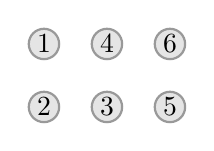
\begin{tikzpicture}
			\node[r](1) at (0,0){1};
			\node[r](2) at (0*\dist,-\disty){2};
			\node[r](3) at (1*\dist,-\disty){3};
			\node[r](4) at (1*\dist,0){4};
			\node[r](5) at (2*\dist,-\disty){5};
			\node[r](6) at (2*\dist,0){6};
		\end{tikzpicture}
		%\subcaption{}
		\subcaption{Initialization.}
		\label{fig:tree0}
	\end{minipage}
	%
	\begin{minipage}[t]{.4\linewidth}
		\centering
		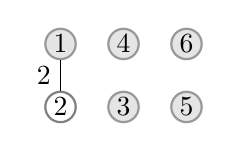
\begin{tikzpicture}
			\node[r](1) at (0,0){1};
			\node[n](2) at (0*\dist,-\disty){2};
			\node[r](3) at (1*\dist,-\disty){3};
			\node[r](4) at (1*\dist,0){4};
			\node[r](5) at (2*\dist,-\disty){5};
			\node[r](6) at (2*\dist,0){6};
			\draw(1)edge node[left]{2} (2);
		\end{tikzpicture}
		%\subcaption{}
		\subcaption{\merge{$2,1,2$}.}
		\label{fig:tree1}
	\end{minipage}

	\vspace{.5cm}
	\begin{minipage}[t]{.4\linewidth}
		\centering
		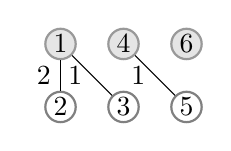
\begin{tikzpicture}
			\node[r](1) at (0,0){1};
			\node[n](2) at (0*\dist,-\disty){2};
			\node[n](3) at (1*\dist,-\disty){3};
			\node[r](4) at (1*\dist,0){4};
			\node[n](5) at (2*\dist,-\disty){5};
			\node[r](6) at (2*\dist,0){6};
			\draw(1)edge node[left]{$2$}(2);
			\draw(1)edge node[left]{$1$}(3);
			\draw(4)edge node[left]{$1$}(5);
		\end{tikzpicture}
		%\subcaption{}
		\subcaption{\merge{$3,2,1$}, then \merge{$5,4,1$}.} \label{fig:T*}
		\label{fig:tree2}
	\end{minipage}
	%
	\begin{minipage}[t]{.4\linewidth}
		\centering
		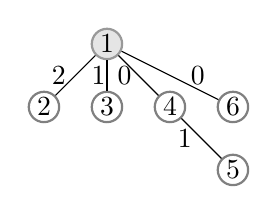
\begin{tikzpicture}
			\node[r](1) at (0,0){1};
			\node[n](2) at (-1*\dist,-\disty){2};
			\node[n](3) at (0*\dist,-\disty){3};
			\node[n](4) at (1*\dist,-\disty){4};
			\node[n](5) at (2*\dist,-2*\disty){5};
			\node[n](6) at (2*\dist,-\disty){6};
			\draw(1)edge node[left]{$2$}(2);
			\draw(1)edge node[left, xshift=3pt]{$1$}(3);
			\draw(1)edge node[left, xshift=1pt]{$0$}(4);
			\draw(1)edge node[right, xshift=4pt]{$0$}(6);
			\draw(4)edge node[left]{$1$}(5);
		\end{tikzpicture}
		%\subcaption{}
		\subcaption{\merge{$4,1,0$}, then \merge{$4,6,0$}.} \label{fig:T*}
		\label{fig:tree3}
	\end{minipage}
	\caption{
		Construction of a rooted tree that represents the hierarchical clustering solution, where a root node is
		highlighted in gray. (a) Initially, we start with an empty forest without edges where each node is a root. (b), (c), and (d) show different stages of building the tree according to
		Algorithm~\ref{algo:aic-tree}. (d) is the final tree representing the clustering solution. Now,
		for any $`g$, the clustering solution can be obtained from the tree in (d) according to Definition~\ref{def:data-structure}, i.e., by removing all
		edges of weight $\leq \gamma$ and returning the connected components as the clustering
		solution. 
		%(a) Initializaiton 
		%(b) \merge{$2,1,2$};
		%(c) \merge{$3,2,1$} \merge{$5,4,1$};
	}
	\label{fig:eg-data}
\end{figure}

	Consider our running example~\eqref{eq:eg-motivate} with $V = \Set{1,\ldots,6}$.
	In Algorithm~~\ref{algo:aic-tree}, the function \initialize{} results in the empty forest in Fig.~\ref{fig:tree0}, where each node is a root, i.e., \Parent{$i$}~$ = i$ for
	$i\in V$. (A root is highlighted in gray.)
	After initialization, the function
	\getPartition{$-\infty$} returns the singletons partition $\mcP = \Set{\Set{i}\mid i \in V}$ of size
	$k = 6$ since initially \Weight{$i$}~$ = -\infty$, for $i\in V$, and so the only node reachable
	from $i$ is node $i$ itself. Subsequently, the algorithm computes the minimum norm base
	$\DataSty{x}[j]$, whose minimum entry is given as
	$\DataSty{x}[j][i] = -2$ for $j \in C_1 = \Set{1}, i\in C_2 = \Set{2}$,
	as we saw in Example~\ref{eg:IC*}, resulting in $\gamma = 2$. Now, the algorithm updates the tree by calling
	\merge{$2,1,2$}, which sets \Parent{$2$}~$ = 1$, \Weight{$2$}~$ = 2$, \Children{$1$}~$ = \Set{2}$,
	\Rank{$1$}~$=1$, and leaves all other variables unchanged. See Fig.~\ref{fig:tree1}.

	Next, the function
	\getPartition{$-\infty$} returns the partition $\mcP = \Set{\Set{1,2}, \Set{3},
	\Set{4}, \Set{5}, \Set{6}}$ (corresponding to the connected components in~\ref{fig:tree1}) of size
	$k = 5$.
	%since $\Weight{$2$} = 2 > -1$ and $\Weight{$i$} = -\infty$ for $i\in V \backslash \Set{2}$. 
	Subsequently, the algorithm computes the minimum norm base
	$\DataSty{x}[j]$, whose minimum entry is given as
	$\DataSty{x}[j][i] = -1$ for $j \in C_1 = \Set{1,2}$ and $i\in C_2 = \Set{3}$,
	and for $j \in C_3 = \Set{4}$ and $i\in C_4 = \Set{5}$,
	as we saw in Example~\ref{eg:thms}, resulting in $\gamma = 1$. Now, the algorithm updates the tree by calling
	\merge{$3,2,1$}, which sets \Parent{$3$}~$ = 1$, \Weight{$3$}~$ = 1$, \Children{$1$}~$ = \Set{2,3}$,
	and leaves all other variables unchanged. (Equivalently, one may call
	\merge{$3,1,1$}, which leads to the same result.)
	The algorithm then calls \merge{$5,4,1$}, which sets \Parent{$5$}~$ = 4$, \Weight{$5$}~$ = 1$,
	\Children{$4$}~$ = \Set{5}$, \Rank{$4$}~$ = 1$, 
	and leaves all other variables unchanged.
	See Fig.~\ref{fig:tree2}. 

	Next, the function
	\getPartition{$-\infty$} returns the partition $\mcP = \Set{\Set{1,2,3}, \Set{4,5}, \Set{6}}$
	(corresponding to the connected components in~\ref{fig:tree2})
	of size $k = 3$. 
	Subsequently, the algorithm computes the minimum norm base
	$\DataSty{x}[j]$, whose minimum entry is given as
	$\DataSty{x}[j][i] = 0$ for $j \in C_1 = \Set{1,2,3}$ and $i\in C_2 \cup C_3 = \Set{4,5,6}$,
	and for $j \in C_2 = \Set{4,5}$ and $i\in C_3 = \Set{6}$,
	as we saw in Example~\ref{eg:thms}, resulting in $\gamma = 0$. Now, the algorithm updates the tree by calling
	\merge{$4,1,0$}, which sets \Parent{$4$}~$ = 1$, \Weight{$4$}~$ = 0$, \Children{$1$}~$ = \Set{2,3,4}$, \Rank{$1$}~$ = 2$
	and leaves all other variables unchanged.
	%(Equivalently, one may call \merge{$3,1,1$}, which leads to the same result.)
	The algorithm then calls \merge{$4,6,0$}, which sets \Parent{$6$}~$ = 1$, \Weight{$6$}~$ = 0$,
	\Children{$1$}~$ = \Set{2,3,4,6}$, and leaves all other variables unchanged.
	See Fig.~\ref{fig:tree3}. 

	Finally, the algorithm terminates upon calling the function \getPartition{$-\infty$} which returns the
	partition $\mcP = \Set{V}$ of size $k=1$.
\end{example}

